\documentclass[a4paper]{article}

\usepackage{graphicx}
\usepackage{float}
\usepackage{a4wide}

\begin{document}

\begin{center}
	\begin{figure}[H]
		\centering
		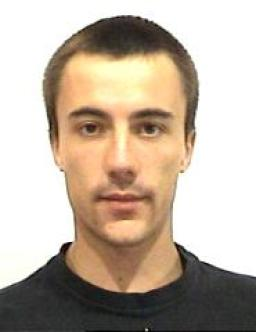
\includegraphics[height=6cm]{jacques}
	\end{figure}
\end{center}

\section*
{
	\Huge{Jacques Lewis}
}
\vspace{0.5cm}

\section*{Contact}
	\begin{description}
		\item[E-Mail:] u28183488@tuks.co.za
		\item[Cell:] (+27) 84 581 0555
		\item[Skype:] i.am.jacques
	\end{description}

\section*{Skills}

	\subsection*{Programming}
		\begin{description}
			\item[C\#:]Solid, 3 years practical experience
			\item[c++:]Solid, 1 year practical experience
			\item[Java:]Solid, 2 years practical experience
			\item[Php:]Moderate, 1 year practical experience
			\item[Delphi]Moderate, 1 year practical experience
		\end{description}
	\subsection*{Databases}
		\begin{description}
			\item[SQL Server:]Solid, 3 years practical experience
			\item[Oracle PL/SQL]Solid, 3 years practical experience
			\item[MySql:]Solid, 2 years practical experience
		\end{description}
	\subsection*{Web}
		\begin{description}
			\item[HTML,CSS,JavaScript:]Solid, 2 years practical experience
			\item[jQuery]Moderate, 1 year practical experience
			\item[ASP.NET]Moderate, 1 year practical experience
			\item[JEE]Limited, less than 1 year practical experience
		\end{description}
	\subsection*{Other}
		\begin{description}
			\item[OpenCV]Limited, I have only recently began playing around with it in my spare time
			\item[Android]Moderate, I am busy with an online course through the Coursera network
		\end{description}
	


\section*{Work Experience}

	\subsection*{2008}
		In my first year after finishing school I was fortunate enough to be employed as a junior software developer at Face Technologies. 
		I was responsible for odd jobs, one of my achievements was reading data from a large, complex flat file into a database.
	\subsection*{2009 - 2011}
		I have always wanted to become a pilot. I left my job at Face Technologies to persue a career in aviation. I worked full time at
		Flight Training Services, a flight school operating out of Grand Central airport in Midrand. My job was to assist customers with
		booking their training sessions, answering phones, managing the aircraft maintenance cycles as well as managing the booking sheets.
	\subsection*{2011 - present}
		I am very thankfull to have been given the opportunity to study towards a degree in Computer Science. I have always been drawn to programming
		and this was an opportunity to further my career. As well as beginning my studies, I was fortunate enough to get a recurring holiday job as
		a student developer at e-Logics. I have worked on many projects during the course of all my visits there, and have progressed to a point where I
		became a recognised developer in a big team. I have learnt a lot during my time there.

\section*{Other Information}

	\subsection*{My Career Plan}
	
	I am very lucky to have the work experience that I do, however that has brought me to the conclusion that I am not entirely stimulated by forms-applications development.
	I like the technical, lower level stuff. My ideal job would involve developing automated systems that make use of computer vision technologies. 

	\subsection*{Interests}
	
	My dream is to develop an autonomous aerial surveilance system that can be used to locate downed aircraft in remote locations. In 2012 a father and son dissappeared 
	in their small aircraft, somewhere over the jungles of Mozambique. I remember following the story, and witnessed how much effort and time was spent in the search operation.
	I imagined how ,maybe, a bunch of drones could be utilised to fly search patterns over the jungle, with an onboard computer vision system scanning the trees below, looking to
	recognise what could be a possible crash site, and then reporting the position back to a command centre. I hope to one day develop such a platform.

\end{document}